% \iffalse
\let\negmedspace\undefined
\let\negthickspace\undefined
\documentclass[beamer]{IEEEtran}
\usepackage{cite}
\usepackage{amsmath,amssymb,amsfonts,amsthm}
\usepackage{algorithmic}
\usepackage{graphicx}
\usepackage{textcomp}
\usepackage{xcolor}
\usepackage{txfonts}
\usepackage{listings}
\usepackage{enumitem}
\usepackage{mathtools}
\usepackage{gensymb}
\usepackage{comment}
\usepackage[breaklinks=true]{hyperref}
\usepackage{tkz-euclide} 
\usepackage{listings}
\usepackage{gvv}                                        
\def\inputGnumericTable{}                                 
\usepackage[latin1]{inputenc}                                
\usepackage{color}                                            
\usepackage{array}                                            
\usepackage{longtable}                                       
\usepackage{calc}                                             
\usepackage{multirow}                                         
\usepackage{hhline}                                           
\usepackage{ifthen}                                           
\usepackage{lscape}
\usepackage[export]{adjustbox}

\newtheorem{theorem}{Theorem}[section]
\newtheorem{problem}{Problem}
\newtheorem{proposition}{Proposition}[section]
\newtheorem{lemma}{Lemma}[section]
\newtheorem{corollary}[theorem]{Corollary}
\newtheorem{example}{Example}[section]
\newtheorem{definition}[problem]{Definition}
\newcommand{\BEQA}{\begin{eqnarray}}
\newcommand{\EEQA}{\end{eqnarray}}
\newcommand{\define}{\stackrel{\triangle}{=}}
\theoremstyle{remark}
\newtheorem{rem}{Remark}
\begin{document}
\parindent 0px
\bibliographystyle{IEEEtran}

\title{GATE - BM 41}
\author{EE23BTECH11215 - Penmetsa Srikar Varma$^{}$% <-this % stops a space
}
\maketitle
\newpage
\bigskip

\renewcommand{\thefigure}{\theenumi}
\renewcommand{\thetable}{\theenumi}
\section*{Question}
Q41) A filter designed using op-amps, resistors and capacitors as shown in figure.
op-amps are ideal with infinite gain and infinite bandwidth. If $\frac{\text{V}_0\brak{\text{s}}}{\text{V}_\text{i}\brak{\text{s}}}$ is an all-pass transfer function, the value of resistor R2 \brak{\text{in k}\Omega} is\\
\begin{figure}[htbp]
    \centering
    \hspace*{-1.8cm}
    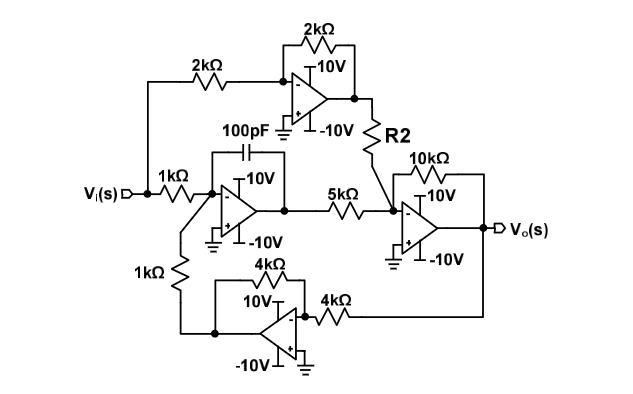
\includegraphics[scale=0.55]{figs/bm,41.png}
    \label{bm,41}
\end{figure}
\begin{center}
\end{center}
\brak{\text{A}}\ 1\\
\brak{\text{B}}\ 10\\
\brak{\text{C}}\ 5\\ 
\brak{\text{D}}\ 2\ \qquad\qquad\qquad\quad\qquad\qquad\qquad\qquad\brak{\text{GATE BM 2022}}
\section*{Solution}
\begin{table}[h]
    \centering
    \begin{tabular}{|c|c|}
     \hline
       variables & conditions  \\
     \hline
         voltage at node 1 & -$\text{V}_{\text{i}}\brak{\text{s}}$ \\
     \hline
         voltage at node 2 & $\text{V}_{\text{0}}\brak{\text{s}}$ \\
     \hline
         voltage at node 3 & $\text{V}_{\text{x}}$ \\
     \hline
         voltage at remaining nodes & 0 V \\
     \hline
         C & capacitor of 100pF \\
     \hline
         $\frac{1}{\text{sC}}$ & laplace domain of capacitor\\
     \hline
        H\brak{\text{s}}=$\frac{\text{V}_0\brak{\text{S}}}{\text{V}_\text{i}\brak{\text{S}}}$ & transfer function\\
     \hline
          $\text{s}_1$ & root of transfer function\\
     \hline
          $\text{s}_2$ & pole of transfer function\\
     \hline
         $\text{R}_2$ & unknown \\
     \hline  
    \end{tabular}

    \label{table}
\end{table}
\begin{center}
    Table of Parameters
\end{center}

for op-amp at $\text{V}_{\text{0}}\brak{\text{s}}$, \brak{\text{we assume $\text{R}_2$ in k$\Omega$}}
\begin{align}
\label{1}
\text{V}_\text{x}&=\frac{5\text{V}_{\text{i}}\brak{\text{s}}}{\text{R}_2}-\frac{\text{V}_0\brak{\text{s}}}{2}
\end{align}

for op-amp at $\text{V}_{\text{i}}\brak{\text{s}}$,
\begin{align}
\label{2}
\text{V}_\text{x}&=\text{sC}\brak{\frac{\text{V}_\text{0}\brak{\text{s}}-\text{V}_\text{i}\brak{\text{s}}}{1000}}
\end{align}

from \brak{\ref{1}} and \brak{\ref{2}} transfer function is given by,
\begin{align}
\text{H}\brak{\text{s}}&=2\brak{\frac{\text{5000+sC$\text{R}_2$}}{\text{1000+2sC}}}
\end{align}
we can observe that for transfer function,
\begin{align}
    \text{s}_1&=-\frac{5000}{\text{C$\text{R}_2$}},\ \text{s}_2=-\frac{1000}{\text{2C}}
\end{align}
since, for all-pass transfer function $\text{s}_1$=$\text{s}_2$,
\begin{align}
    \text{R}_2&=\text{10 k}\Omega
\end{align}
so, option B is correct
\end{document}
